% This work is made available under the terms of the
% Creative Commons Attribution-ShareAlike 4.0 license,
% http://creativecommons.org/licenses/by-sa/4.0/.
%
% Version: $Revision: 4890 $

\documentclass[a4paper]{book}

\usepackage{wrapfig}
\usepackage{graphicx}
\usepackage{hyperref}
\usepackage{multirow}
\usepackage{scalefnt}
\usepackage{tikz}

% watermark -- for draft stage
\usepackage[firstpage]{draftwatermark}
\SetWatermarkLightness{0.9}
\SetWatermarkScale{5}

% Copyright (c) 2009 by the University of Waikato, Hamilton, NZ. 
% This work is made available under the terms of the 
% Creative Commons Attribution-ShareAlike 3.0 license, 
% http://creativecommons.org/licenses/by-sa/3.0/. 
%
% Version: $Revision$

\newenvironment{tight_itemize}{
\begin{itemize}
  \setlength{\itemsep}{1pt}
  \setlength{\parskip}{0pt}
  \setlength{\parsep}{0pt}}{\end{itemize}
}

\newenvironment{tight_enumerate}{
\begin{enumerate}
  \setlength{\itemsep}{1pt}
  \setlength{\parskip}{0pt}
  \setlength{\parsep}{0pt}}{\end{enumerate}
}

% if you just need a simple heading
% Usage:
%   \heading{the text of the heading}
\newcommand{\heading}[1]{
  \vspace{0.3cm} \noindent \textbf{#1} \newline
}

\newcommand{\icon}[1]{\tikz[baseline=-3pt]\node[inner sep=0pt,outer sep=0pt]{\includegraphics[height=1.1em]{#1}};}


\title{
  \textbf{ADAMS} \\
  {\Large \textbf{A}dvanced \textbf{D}ata mining \textbf{A}nd \textbf{M}achine
  learning \textbf{S}ystem} \\
  {\Large Module: adams-event} \\
  \vspace{1cm}
  
\includegraphics[width=2cm]{images/event-module.png} \\
}
\author{
  Peter Reutemann
}

\setcounter{secnumdepth}{3}
\setcounter{tocdepth}{3}

\begin{document}

\begin{titlepage}
\maketitle

\thispagestyle{empty}
\center
\begin{table}[b]
	\begin{tabular}{c l l}
		\parbox[c][2cm]{2cm}{\copyright 2012-2015} &
		\parbox[c][2cm]{5cm}{
\includegraphics[width=5cm]{images/coat_of_arms.pdf}} \\
	\end{tabular}
	
\includegraphics[width=12cm]{images/cc.png} \\
\end{table}

\end{titlepage}

\tableofcontents
\listoffigures
%\listoftables

%%%%%%%%%%%%%%%%%%%%%%%%%%%%%%%%%%%
\chapter{Flow}
The following actors are available:
\begin{tight_itemize}
	\item \textit{TriggerEvent} -- control actor for triggering an event found
	below an \textit{Events} standalone.
	\item \textit{Cron} -- standalone for scheduled events. See \ref{cron} for 
	more details.
	\item \textit{DelayedEvent} -- standalone that executes its sub-flow after
	a predefined number of milli-seconds.\footnote{adams-event-delayed\_event.flow}
	\item \textit{DirWatch} -- standalone that watches a directory for file
	events (create, change, delete).\footnote{adams-event-watch\_dir.flow}
	\item \textit{Events} -- standalone similar to \textit{CallableActors}, used
	for grouping events.
	\item \textit{ExternalStandalone} -- is a triggerable event and can be 
	added to the \textit{Events} standalone.
	\item \textit{Flow} -- a flow itself is a triggerable event as well.
	\item \textit{LogEvent} -- standalone that allows listening to global 
	logging events and processing of the received log records.
	\item \textit{QueueEvent} -- standalone that allows listening to a queue 
	(ArrayList) located in internal storage and process items as soon as they
	become available.
	\item \textit{VariableChangedEvent} -- standalone that allows listening to
	changes to a specific variable.
\end{tight_itemize}

%%%%%%%%%%%%%%%%%%%%%%%%%%%%%%%%%%%
\chapter{Cron jobs}
\label{cron}
Cron jobs are a very convenient way of performing background jobs that are only
executed once in a while at specific times. For instance, a ``clean up'' job 
could run once every night, or a ``backup'' job every Friday night.

The \textit{Cron} standalone can be used to \textit{trigger} and execute these 
jobs. You can either place the actors that the job consists of below the 
\textit{Cron} itself\footnote{adams-event-displaying\_directory\_contents1.flow} 
or place them under a \textit{Flow} control actor inside
the \textit{Events} standalone and call this event then using the 
\textit{TriggerEvent} control 
actor.\footnote{adams-event-displaying\_directory\_contents2.flow}

Since the cron jobs get executed at fixed times, we need to have a flow that is
running forever, unless stopped by the user (or the cron job itself). This can 
be implemented using the \textit{WhileLoop} control actor with an enclosed 
\textit{Sleep actor}. To simplify this setup, there is already a sub-flow 
template available that generates such a flow: \textit{EndlessLoop}.

The format for the cron job execution is not very intuitive when you look at it
for the first time. In order to make it easier, you can use the editor that ADAMS
offers (see Figure \ref{cron-editor}). This editor allows you to check the
current input as well as opening a web page with a detailed description of
the format (see \cite{cronformat}).

\begin{figure}[htb]
  \centering
  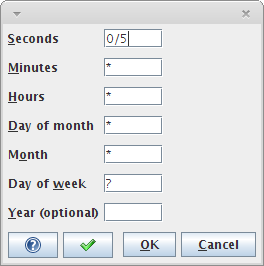
\includegraphics[width=4.0cm]{images/cron-editor.png}
  \caption{The editor for entering the execution time of a cron job.}
  \label{cron-editor}
\end{figure}

%%%%%%%%%%%%%%%%%%%%%%%%%%%%%%%%%%%
% Copyright (c) 2009-2012 by the University of Waikato, Hamilton, NZ. 
% This work is made available under the terms of the 
% Creative Commons Attribution-ShareAlike 4.0 license,
% http://creativecommons.org/licenses/by-sa/4.0/.
%
% Version: $Revision$

\begin{thebibliography}{999}
	% to make the bibliography appear in the TOC
	\addcontentsline{toc}{chapter}{Bibliography}

    % references
	\bibitem{adams}
		\textit{ADAMS} -- Advanced Data mining and Machine learning System \\
		\url{https://adams.cms.waikato.ac.nz/}{}

	\bibitem{esrigrid}
	 	\textit{Esri Grid} -- a raster GIS file format deveoped by Esri. \\
		\url{https://en.wikipedia.org/wiki/Esri\_grid}{}

	\bibitem{kml}
	 	\textit{Keyhole Markup Language} -- an XML notation for expressing
	 	geographic annotation and visualization within Internet-based,
	 	two-dimensional maps and three-dimensional Earth browsers. \\
		\url{http://en.wikipedia.org/wiki/Keyhole\_Markup\_Language}{}

	\bibitem{postgresql}
	 	\textit{PostgreSQL} -- a powerful, open source object-relational
	 	database system. \\
		\url{http://www.postgresql.org/}{}

	\bibitem{postgis}
		\textit{PostGIS} -- a spatial database extender for PostgreSQL
		object-relational database. It adds support for geographic
		objects allowing location queries to be run in SQL.  \\
		\url{http://postgis.net/}{}

	\bibitem{srid4269}
	 	\textit{SRID 4269} -- or NAD 83 (North American Datum). \\
		\url{http://spatialreference.org/ref/epsg/4269/}{}

	\bibitem{mysql}
		\textit{MySQL} -- an open-source relational database management
		system (RDBMS) \\
		\url{http://www.mysql.com/}{}

\end{thebibliography}


\end{document}
